\documentclass[journal]{IEEEtran}

\renewcommand\thesection{\arabic{section}} 
\renewcommand\thesubsectiondis{\thesection.\arabic{subsection}}
\renewcommand\thesubsubsectiondis{\thesubsectiondis.\alph{subsubsection}}
\renewcommand\theparagraphdis{\arabic{paragraph}.}

%\usepackage[retainorgcmds]{IEEEtrantools}
%\usepackage{bibentry}  
\usepackage{xcolor,soul,framed} %,caption

\colorlet{shadecolor}{yellow}
% \usepackage{color,soul}
\usepackage[pdftex]{graphicx}
\usepackage[cmex10]{amsmath}
\usepackage{array}
\usepackage{mdwmath}
\usepackage{mdwtab}
\usepackage{eqparbox}
\usepackage{url}
\usepackage{amsfonts}
\hyphenation{op-tical net-works semi-conduc-tor}
\usepackage{graphicx}
\usepackage{amsmath}
\usepackage{lmodern}
\newtheorem{definition}{Definition}


\usepackage{xcolor}
\definecolor{th}{RGB}{0,83,161}
\graphicspath{{../pdf/}{../jpeg/}}
\DeclareGraphicsExtensions{.pdf,.jpeg,.png}

\usepackage[
    bookmarks=true,
    bookmarksopen=true,
    bookmarksnumbered=true,
    bookmarksopenlevel=1,
    pdfpagelabels=true,
    colorlinks=true,
    linkcolor=th,
    urlcolor=th,
    anchorcolor=th,
    citecolor=th,
    filecolor=th,
    menucolor=th,
    plainpages=false,
    hypertexnames=true,
    linktocpage=false,
]{hyperref}

\usepackage[cmex10]{amsmath}
%Mathabx do not work on ScribTex => Removed
%\usepackage{mathabx}
\usepackage{array}
\usepackage{mdwmath}
\usepackage{mdwtab}
\usepackage{eqparbox}
\usepackage{url}
\hyphenation{op-tical net-works semi-conduc-tor}
\usepackage{graphicx}



%\bstctlcite{IEEE:BSTcontrol}
%=== TITLE & AUTHORS ====================================================================
\begin{document}

\bstctlcite{IEEEexample:BSTcontrol}
	
    \title{    
    
\includegraphics[width=7.5in]{photo/logo.png}
    \newline \newline
     IT-Projekt \\ 
     \textit{Autonmously driving Remote Control Car
     \\ \text{\normalfont\ {\huge with DonkeyCar and Raspberry Pi 3B+}}}
     }

  \author{
      \textbf{L\"OHR} Tim,
      \textbf{BOHNSTEDT} Timo, 
      \textbf{PALPANES} Ioannis
}

% The paper headers
\markboth{IT-Project at the TH-OHM
}{Roberg \MakeLowercase{\textit{et al.}}}


% ====================================================================
\maketitle
% === ABSTRACT 
\begin{abstract}
For our group IT-project at the \textit{University of Applied Science Georg Simon OHM}, we built an autonomously driving remote control car. To accomplish this project, we used the framework \textit{DonkeyCar}. Supervised learning is the primary component, but we provide related work and projects to compare this project with the \textit{state-of-the-art} Reinforcement Learning. We explain how to connect the car with the microcontrollers and cables, to do a full reverse-engineering on project. Every single component will be introduced in an appropriate complexity for non-electrical-engineers.  The neural network is a \textit{VGG16}-Network, which will be explained with all details and parts to understand the networks' architecture fully. We further provide information about how the car can be driving with the webserver. The Report gives a detailed explanation of the API and the transferred data.
\end{abstract}
% === KEYWORDS 
\begin{IEEEkeywords}
\hl{Machine Learning, IT-Project, RC-Car, RaspberryPi, Autonomusly driving}
\end{IEEEkeywords}
\IEEEpeerreviewmaketitle

% === I. Project background and motivation
\section{Project background and motivation}
\label{sec:backgroundMotivation}
We decided to commit ourselves to this kind of project because we are interested in many aspects related to machine learning. We knew that our skills and knowledge were at the starting point not deep enough, but after completing this project within two semesters, we gained a lot of information and understood the details of machine learning more as before. Along the many hours we spent, we had to learn new things, and we can say with some proud that we managed to make the car drive autonomously - with a lot of effort though.
It is known that the car industry(especially in Germany) undergoes a shift towards electric and autonomous-driving cars currently. The old engine-driven vehicles seem to be \textit{outdated technology}. For three eager students who are interested in computer science and everything related to it, a new opportunity arose and is still occurring. Especially in the area of autonomous-driving cars, companies invest a lot of money and time. They also search for talents which could make a difference in the future. It was especially hard, in the beginning, to split the responsibilities and figure out who takes care of which element in the project. Even the first car we bought was not compatible with the hardware we purchased (Raspberry Pi 3B+, Servodriver, e.g.). That did not stop us from learning about the equipment and the software we wanted to use more precisely. How we combine the hardware with the right software, so that the car can move on its own, was one of the most exciting and exciting aspects we wanted to explore.
But in the end, an essential aspect and the reason why we wanted to do the project in the first place, was the software - especially: the neuronal networks, machine- and deep learning software. This area can not only be used for cars and hardware-related problems, but it is also used for understandable software such as movie recommendations in, e.g. the Netflix interface.
The main question we asked ourselves was: \textit{How can we teach our software to steer a car autonomously with the right velocity on a defined road with the help of images we fed into the database?} In the following, we explain to the reader exactly how we did it. We hope the reader enjoys the topic as much as we did along the hard but rewarding way.
\section{Literature Survey}
\label{sec:LiteratureSurvey}
\subsection{The Level of autonomously driving Cars}
Let us start the survey with defining the autonomously driving itself first. Since this kind of driving evolved within a long period of time, different levels of autonomous driving have been invented and get officially declared. 
There are defined five levels of vehicle autonomy from the National Highway and Traffic Safety Administration (NHTSA) \footnote{\url{https://www.truecar.com/blog/5-levels-autonomous-vehicles/}}.

\begin{itemize}
\item \textit{Level 0 - No Automation}: The car is driven by a human
\item \textit{Level 1 - Driver Assistance}: There is a single vehicle control system like steering into the middle of the lane or braking the tires when the distance to the car in front is too close, but only one at a time.
 \item \textit{Level 2 - Partial Automation}: The car performs the accelerating and decelerating by itself. The human is still supposed to look over the environment and be aware of the surroundings. \\
Example: Tesla Autopilot \cite{tesla}	
\item \textit{Level 3 - Conditional Automation}: The autonomous car takes the entire control even under special occurrences like animal on the road. The human is still expected to intervene when it is required. \\
Example: Google Waymo \textit{self-driving car} \cite{google}
\item \textit{Level 4 - High Automation}: The car takes over the entire control of the driving system and the human is not required to pay any attention to the environment. The car is expected to to perform all driving tasks safely and without special circumstances. \\
Example: Waymo announced in 2017 that they are testing \textit{level 4} driving \cite{google2}
\item \textit{Level 5 - Full Automation}: The car takes over the entire control of the driving system and the human is not required to pay any attention to the environment, nor does need to be inside of the car. 
\end{itemize}
\subsection{Reinforcement Learning}
The two significant approaches in the Machine Learning field are supervised and unsupervised learning. Supervised learning requires labelled data, and this means the data is already tagged with the \textit{correct answer}. The model learns on the data and their labels and predicts an output based on that. Whereas the unsupervised learning describes how the model works on its own to discover the information. It deals mostly with unlabeled data and gets penalized if it produces wrong results. Unsupervised learning has some prime advantages over supervised learning:
\begin{itemize}
\item Finds all kind of unknown patterns: Unknown objects on the road, broken streets
\item Optimizes the performance criteria with the use of experience
\item Solves various types of real-world problems, such as autonomous driving
\end{itemize}
We found that a team from the North China University of Technology already approached the try to drive the donkey car autonomously \cite{reinforcement}. The team used the \textit{gym environment} from OpenAI \footnote{\url{https://gym.openai.com/}}. This open-source project from OpenAI allows building relatively easy penalizing models to implement reinforcement Learning. OpenAI provides plenty of API's such as reset(), step() or is\_game\_over(). These methods are the core of the model to recognize its faults. \\
They use the DDQN algorithm to perform reinforcement Learning. DDQN stands for Deep Reinforcement Learning with Double Q-learning \cite{reinforcement2} developed by a team of researchers at \textit{Google DeepMind}. Explaining how this algorithm works would exceed the limits of this paper, but the final output of the team \cite{reinforcement} was autonomously driving donkey car. The training process was fairly slow, and it didn't drive completely exact, but the experiment shows that reinforcement Learning can be implemented together with the donkey car quite easily.
\section{Hardware}
Usually, the car is driven by remote control. Which sends signals to the steer of the wheels depending on which buttons the controlling user pushes. In our case, we want to control the car only with the computer itself. To fulfil that, we will need to buy some extra parts, rewire the remote control car’s servomotor and connect it to the onboard Raspberry Pi 3B computer. We will also need a camera to capture the images and a servomotor controller.
\subsection{RC Car}
Our car is the \textit{s-idee® 18175 9115 RC Car Buggy waterproof monster-truck 1:12}.
The remote control car is the heart of our project. Even though every RC Car can be used to drive autonomously, it is a better choice to buy a real model car, because a real servomotor makes it much easier to connect the pins to. The car’s ESC (electronic speed controller) must be apart from its signal receiver. The steering servo and the ESC must be connectable to the servo motor controller for the Raspberry Pi to control both fully. It is an advantage if the ESC supports fine-tuning of the steering angle to drive the car more precisely. 
The cost of a real model RC car is approximately 100 euros, and so was the price of ours. The car must be quite large because we need to store the Raspberry Pi, the camera and a power bank for the Pi onto the car without losing to much speed of the vehicle. To keep everything in position, we attached it with a 3D print of a plastic holding-system, which was tailored by us for our car. \\
\begin{figure}
  \begin{center}
  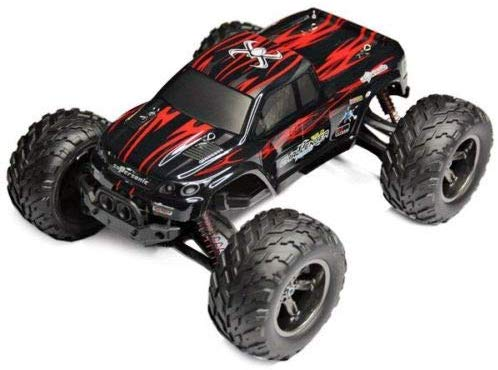
\includegraphics[width=2.5in]{photo/car.jpg}\\
  \caption{Remote Control Car}\label{car}
  \end{center}
\end{figure}
\subsubsection{Technical Details}
Our car comes with 2,4 GHz type of remote control and is 40 km/h fast. It only weights 1,88 Kg. Since the vehicle is typically steered by the remote control, in our case, we use the Raspberry Pi to drive it autonomously. The battery is a 9,6V with 800 mah, which gives us plenty of time to capture pictures of the track to train the model. The car-like casing is easy to remove, to attach the Raspberry Pi and the rest onto it.
\subsubsection{Servomotor}
The servomotor is the key to connect the Raspberry Pi with the RC car. A normal servomotor has two times three pins attached to it. One responsible for the steering and the other one for the speed. The steering is managed by a so-called PWM (Pulse Width Modulation), as shown in figure \ref{pwm}. Depending on the length of the signal, the steering performs a certain degree of changing its angle. We need to configure and set up the optimum values for our car in the Python \textit{steering} file.\\
\begin{figure}
  \begin{center}
  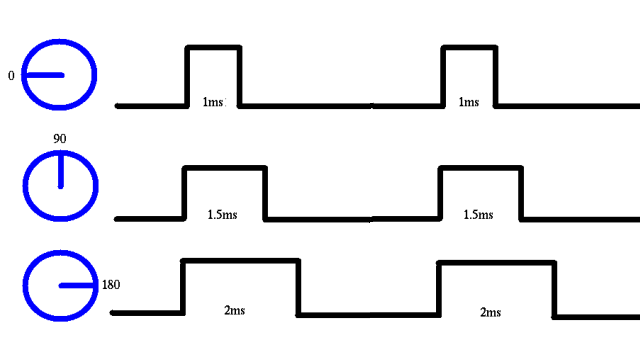
\includegraphics[width=2.5in]{photo/pwm}\\
  \caption{PWM signal}\label{pwm}
  \end{center}
\end{figure}
\subsection{Raspberry Pi}
Our group project aims to be affordable, so we chose the Raspberry PI 3 Model B+. There would be a better onboard computer such as the \textit{NVIDIA DRIVE PX Pegasus} for larger projects, but the computing power exceeds our requirements by far.
Even though by now the Raspberry Pi 4 is out, we still use the Raspberry Pi 3B+, because we are sure that it is compatible with our other microcontrollers and software. \\
We use a 16GB SanDisk to store the operating system and the machine learning model on the Raspberry Pi. \\
\subsubsection{Technical Details}
The Raspberry Pi 3B+ is equipped with a lot of different extensions. It has a Wi-Fi module to communicate with the Python web server and a fairly fast processor to run the neural network and classify where to drive next. The Processor is the Broadcom BCM2837B0, Cortex-A53 with 1.4GHz and it has 1GB LPDDR2 SDRAM. \\
Furthermore, for the connectivity, the Pi has extended 40-pin GPIO headers. The weight is only 42 grams, which makes it easy to attach it onto the RC car. The \textit{Donkey Car Project} \cite{donkey} provides a prepared operating system for the Raspberry Pi called \textit{donkeypi}. This OS is based on the basic \textit{raspbian OS} from the Raspberry Pi company, but also includes the prepared Python files to start the webserver, read in the images and drive autonomously based on the images classified through the trained model. \\
\subsubsection{Cameramodule}
\label{sec:cameramodule}
For our purpose, we use the Raspberry Pi Camera Module 8MP v2.1. It can capture pictures with 1080p and 8-megapixel focus. 
It is straightforward to plug the camera onto the Raspberry Pi. The camera connects directly into the CSI (Camera Serial Interface) connector on the Raspberry Pi with a 15 pin Ribbon Cable. The CSI Bus can easily handle 20 to 30 FPS (frames per second). The weight of 3 grammes makes no difference for the RC Car. \\
\begin{figure}
  \begin{center}
  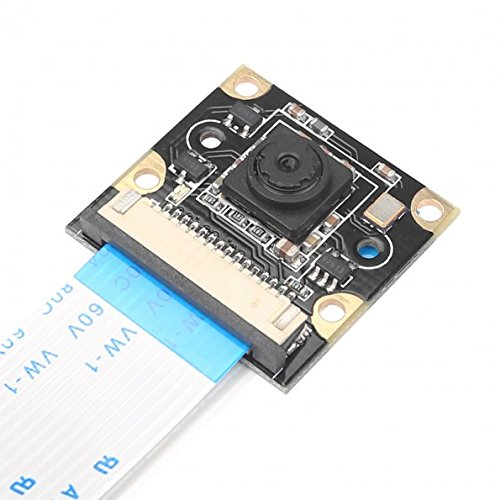
\includegraphics[width=1.5in]{photo/camera.jpg}\\
  \caption{Raspberry Pi Camera Module}\label{camera}
  \end{center}
\end{figure}

We are not required to use a wider lens because our test track is big enough. The images captured by this camera are sequential to the input for the model to train. 1080p is relatively large and would take an eternity to train; this is why we need to scale the image down to 160x120 pixels. Furthermore, we use a framerate of 20, which means we capture 20 images per second.  

\subsection{Servodriver}
We use SunFounder PCA9685. The price for this microcontroller is approximately 13 euro on the most famous marketplaces. The servo driver is needed to produce the PWM (Pulse width modulation) signals for our Raspberry Pi. It acts as joint for the RC cars' servomotor and the Raspberry Pi. \\

\begin{figure}
  \begin{center}
  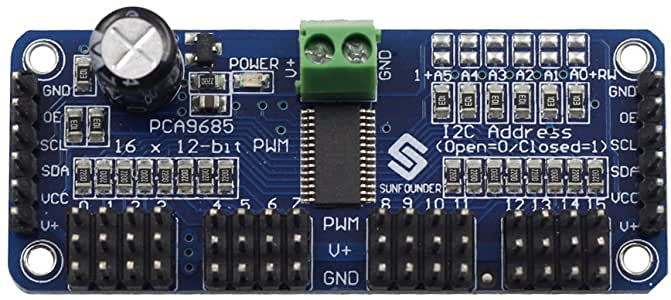
\includegraphics[width=2.5in]{photo/sunfounder.jpeg}\\
  \caption{SunFounder PCA9685}\label{servodriver}
  \end{center}
\end{figure}

\subsubsection{Technical Details}
he SunFounder PCA9685 consists of many different Pins \cite{servo}. The GND and the VCC pin to power it. The VCC has used the voltage of 3-5V. Furthermore are three control pins on the board, namely the:

\begin{itemize}
\item SCL - I2C clock pin
\item SDA - I2C data pin 
\item OE - Output enable 
\end{itemize}

\subsection{Cable Management and Battery}
\subsubsection{Servomotor to Servodriver}
A real model car always has a servomotor as a motor. This servomotor receives input from two pins, and each of the two is powered separately with V+ and the GND pin. 
So in total, the servomotor has six pins. Whereas the servo driver has 3x16 rows of pins available on it.  The three following pins are responsible for the output:

\begin{itemize}
\item V+ - Power supply
\item GND - Ground
\item PWM
\end{itemize}

We connect the servomotor pins accordingly onto two of the rows of the servo driver. This six pins in total control the entire behaviour of the car. One of the three-pin-blocks is responsible for the steering, and the other one is responsible for the speed of the vehicle. \\

\begin{figure}
  \begin{center}
  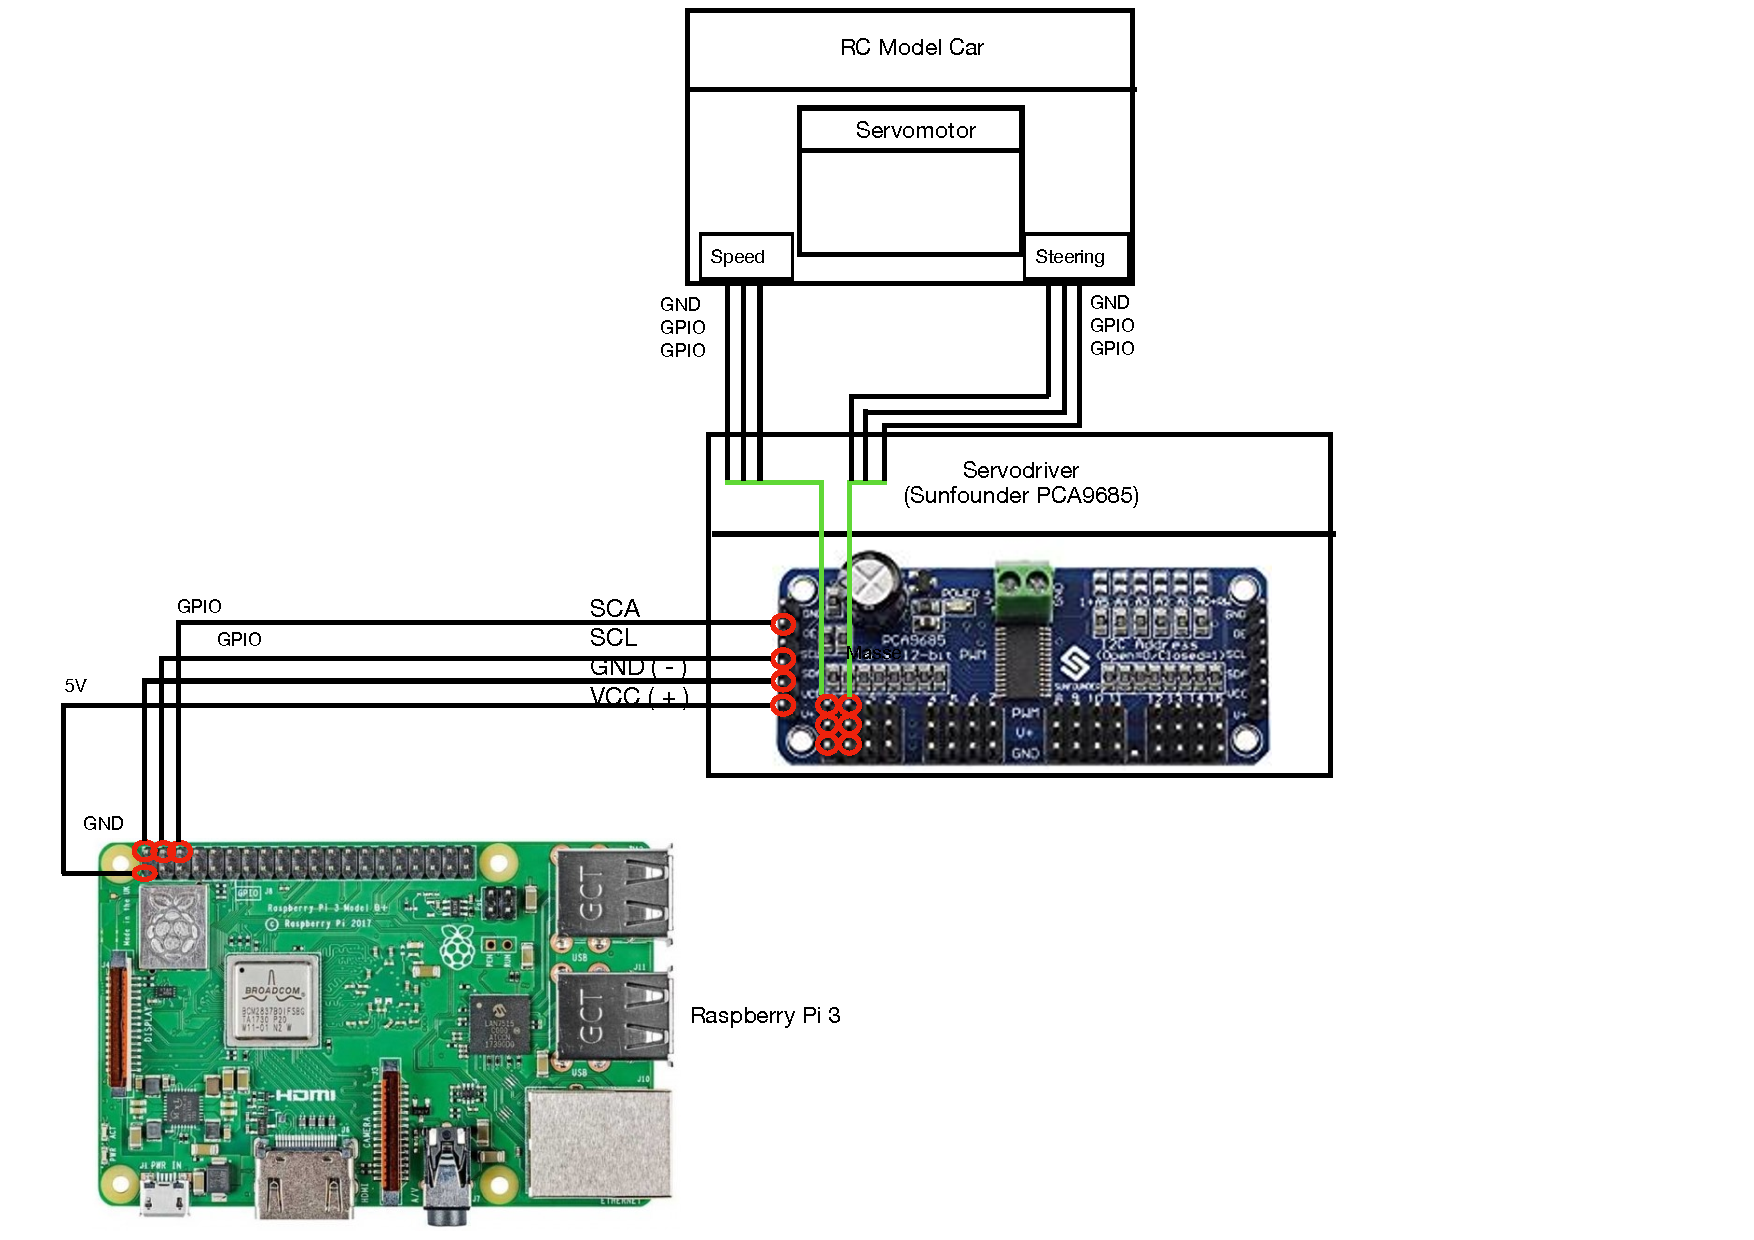
\includegraphics[width=3.5in]{photo/ebene2.pdf}\\
  \caption{Cable Management}\label{ebene2}
  \end{center}
\end{figure}

\subsubsection{Servodriver to Raspberry Pi}
There are four pins that we need to connect from the Raspberry Pi onto the servo driver. Two out of those four pins are just for the power supply. We link the 5V pin from the Raspberry Pi to the VCC pins, which accordingly powers the SunFounder servo driver. To make a power supply work, we always need the ground pin (GND) as well. The other two pins communicate the data from Raspberry Pi to servo driver and vice versa. The communication pins work with the I2C bus system, which is used by the SDL (serial data) pin and the SCL (serial clock). The SDL 10Bit addressing bus sends the data, and the SCL sets up the clocking time, respectively. Both the Raspberry Pi and the servo driver have the SDL and the SCL connector pins, so we can easily plug them in. 
\subsubsection{Battery}
The Raspberry Pi 3 Model B+ has an optimum power supply of 5V and 2.1A.  A power bank is responsible for the power of the vehicle.  We use the power bank from the company \textit{Anker} with \textit{20000mAh}. It provides a 2.1A and 5V output which fully fulfils all the Raspberry Pi's power requirements. \\
\section{Software Architecture}

In this section, we give a quick overview of how the entire software is connected (Figure \ref{webserver}). The following UML diagram shows the whole flow of the data.

\begin{figure}
  \begin{center}
  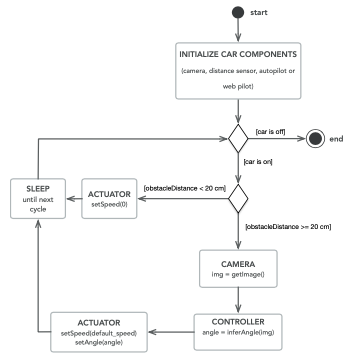
\includegraphics[width=3in]{photo/uml}\\
  \caption{UML Diagram from David Ungurean \cite{master}}\label{uml}
  \end{center}
\end{figure}

\subsection{Python Files}

The \textit{Donkey Self-Driving Car} \cite{donkey} Project is the basis for our group Project. So,  we are constraint to use the same folder structure, which is:

\begin{itemize}
\item management
\item parts
\item templates
\item test
\end{itemize}

Whereas management includes everything related to the webserver (as explained in the next subsection). The parts folder contains all the single devices related to getting the car to drive by itself. Included in the parts folder is, e.g. Pi Camera module, the Keras neural network and the image configurations to use them as input for the neural network. 

\subsection{Webserver}

For the web server we use the Python \textit{package} called \textit{Tornado}. Tornado is a basic multi-purpose WebSocket which is open-source to use. The Tornado helds the bidirectional communication between the server and the browser. To receive the live transmission of the pictures of the camera module, we use the Tornado web server. As shown in figure \ref{ebene2}, we access the webserver over the \textit{localhost} and the \textit{Port 37}. This Port is standardized by IEEE \footnote{\url{https://de.wikipedia.org/wiki/Liste_der_standardisierten_Ports}} as the \textit{TIME Protocol} and fits perfect to our requirements for tracking time intervals.

\begin{figure}
  \begin{center}
  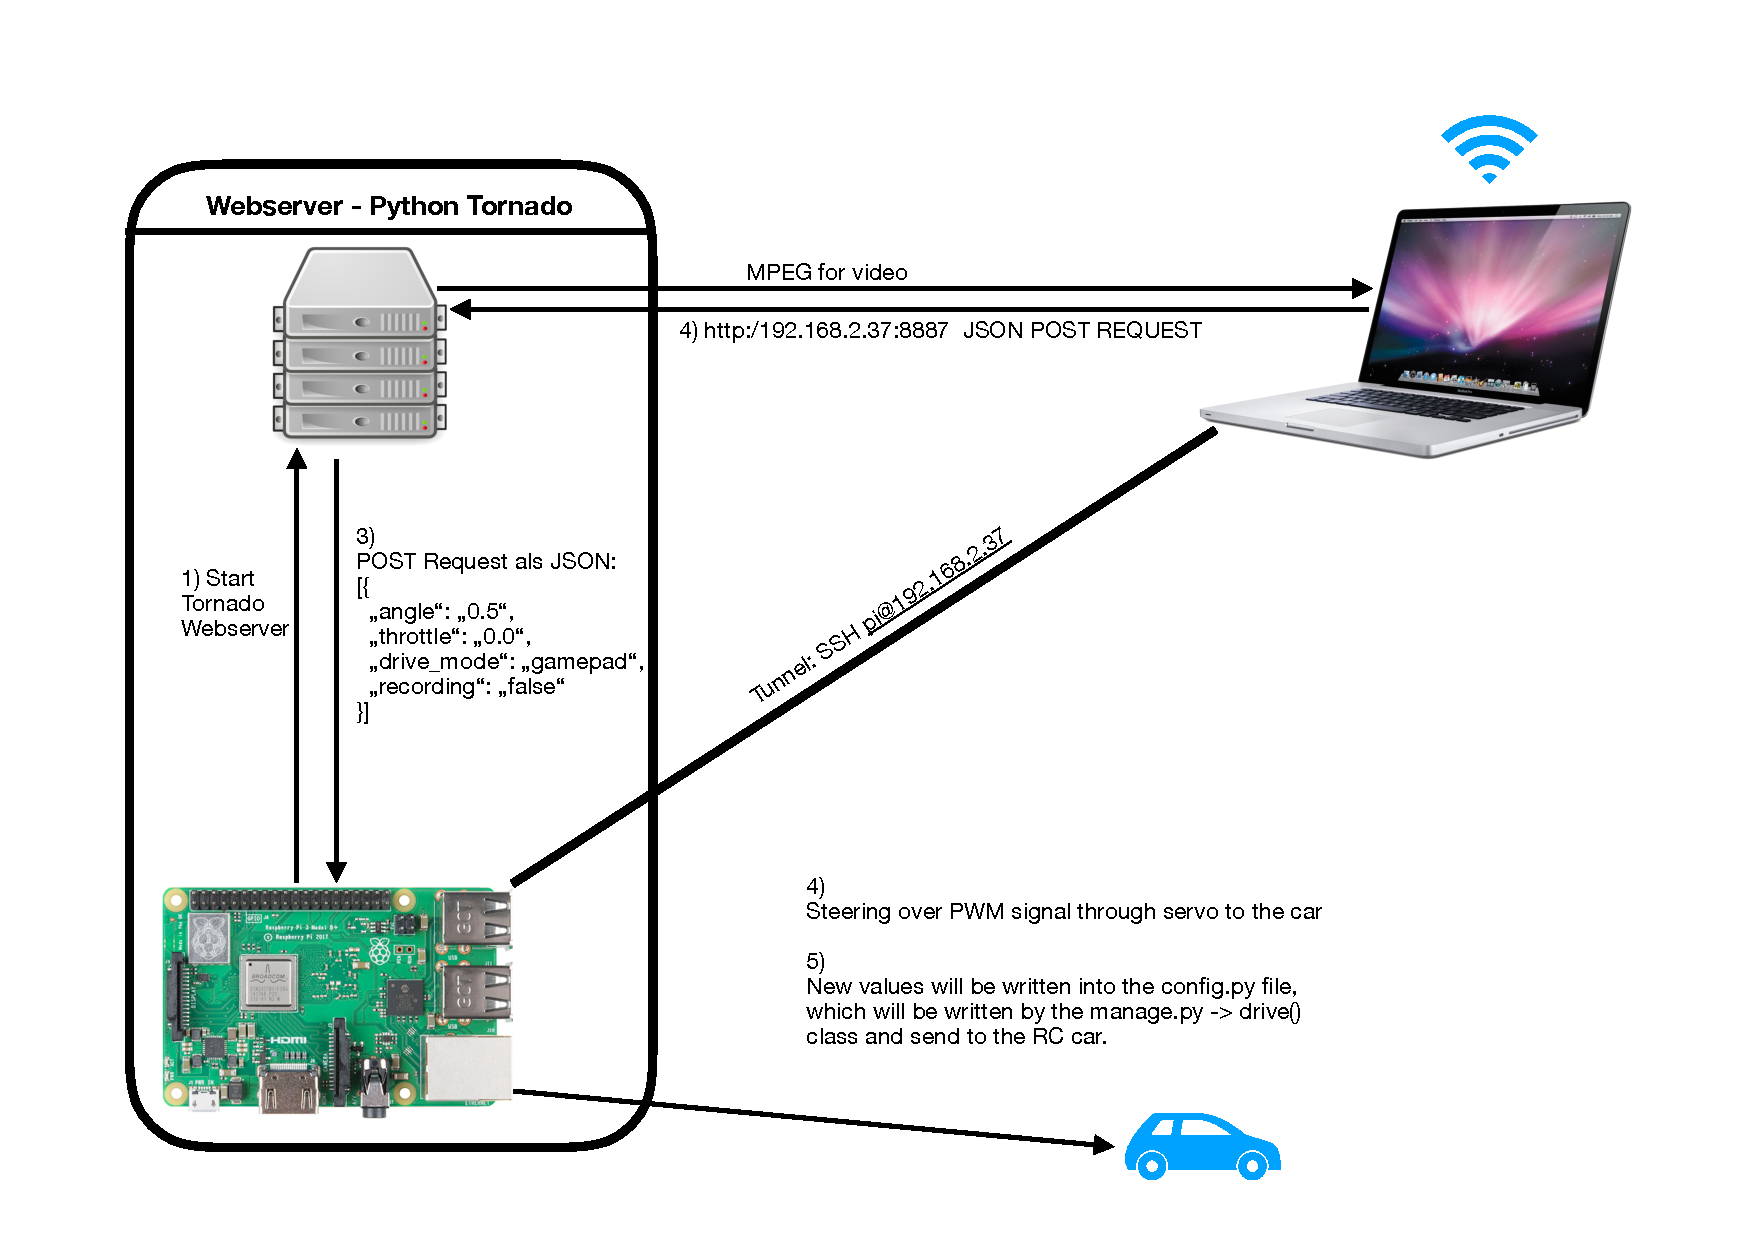
\includegraphics[width=3.5in]{photo/webserver.pdf}\\
  \caption{Webserver Overview}\label{webserver}
  \end{center}
\end{figure}

\subsection{Unity}

Based on the work of the open-source developer project from Twan Kramer, donkey car provides a simulator software. The Simulator allows us to drive with the car as with a real RCC\-Car. While driving, we can record labelled pictures. The C\# Framework Unity is building used to implement the simulator software. More precisely, it uses the Unity 3D game engine to simulate car physics in a 3D world and generates image steering pairs to train our neural network \cite{sdsandbox}. In the Simulator, we can choose between different environments. So, we can be sure that the generated data has enough variety to get a useful model \cite{contributionOfVariables}. Going on a more detailed level would be too much to provide all those details in our report. 

\section{Machine Learning}
As mentioned in our Project \hyperref[sec:backgroundMotivation]{background and motivation section}, machine learning is the heart of our project. So, before we are diving deeper into the details, we want to give a small overview of this topic. Machine Learning includes a large variety of techniques. Those techniques used for building programs which can use the experience to apply them on specific tasks. In other words, formally described as: \\
\begin{definition}
\noindent"A computer program is said to learn from experience E with respect to some class of tasks T and performance measure P, if its performance at tasks in T, as measured by P, improves with experience E"\- Mitchell (1997)  \\
\end{definition}
Experience can be seen as training data \cite{wang_2003} so that it is not necessary to programme all possible cases by hand. To program, all possible scenarios like in earlier introduced chess computers would not work \cite{Goodfellow-et-al-2016}. That it is not possible to program, all possible scenarios are especially true for unstructured data. Unstructured data is data that isn't easy to store in a spreadsheet. For example, it could be an image, sound or text. Unstructured data is hard to interpret for computers \cite{Goodfellow-et-al-2016}\cite{LeCun1998}. In the last years, three major changes made it possible that computers are getting better in interpreting unstructured data. First, we had more data which could be used to work on different projects. Second, we know more efficient Algrorythmes as before, because of the research which happens in the last years.
Last but not least was an increase of computational potential. It is essential to say that this happened mostly not because of better hardware itself. Responsible is more a more advanced parallelisation technique running on the equipment. Besides the different data types like structured and unstructured data, plenty of tasks could be solved with machines which can learn from experience. To get a self-driving car, we must answer an image classification task. The camera fixed on the case of our car records images and sent them directly to the board computer. The computer has now to decide in which direction it should drive. The computers decision is based on the objects he could "see" on the picture. I more detailed and technical explanation on is given in the \hyperref[subsec:deeplearning]{Deep Learning Subsection} and the \hyperref[sec:AutonomouslyDriving]{Autonomously Driving Section}.
\subsection{Deep Learning}
\label{subsec:deeplearning}
Deep Learning means we have a deep neuronal network. Per Definition, we get a deep neural network if we had more than one hidden layer in a neural network. Neural Networks are a concept in the machine learning field which try to build a program that learns like the human brain is learning. Like the human brain, such an application is made from so-called neurons. On a very fundamental level, we can say that neurons are functions \cite{RN5}. If you compare the structure of both neurons, the neurons in our brain (figure \ref{fig:bioneuron}
%========================================================================
\begin{figure}
  \begin{center}
  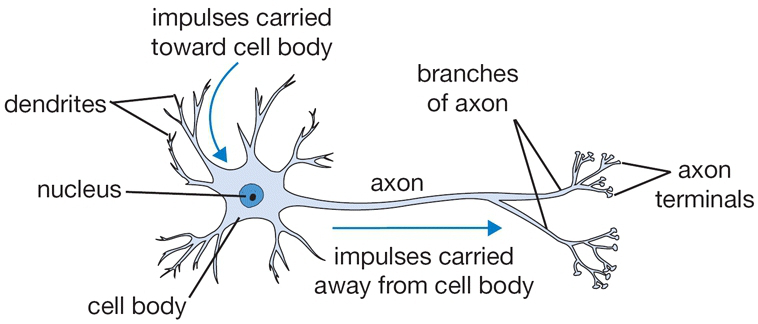
\includegraphics[width=3in]{photo/neuron-brain}\\
  \caption{A cartoon drawing of a biological neuron }
  \label{fig:bioneuron}
  \end{center}
\end{figure}
%========================================================================
and the technical model (figure \ref{fig:mathneuron},
\begin{figure}
  \begin{center}
  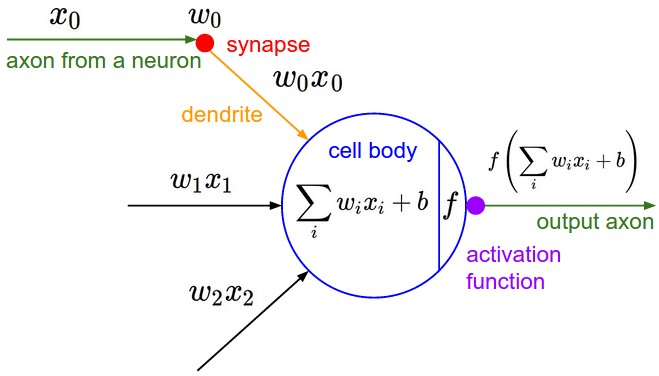
\includegraphics[width=3in]{photo/neuron_model}\\
  \caption{A cartoon drawing of a biological neurons mathematical model}
  \label{fig:mathneuron}
  \end{center}
\end{figure}
%========================================================================
which is used in neural networks, is similar. Besides the shape of the neurons, there are considerable differences in the way the human brain works and the way the deep neural network works. With an increase in the performance of those networks, the idea of rebuilds a human brain is almost gone. Instead, we are using modern mathematical theorems and functions that could solve machine learning tasks faster even we know that it has nothing to do with the human brain. Deep neuronal networks as you can see in figure \ref{fig:neural-network}
%========================================================================
and the technical model (figure \ref{fig:mathneuron},
\begin{figure}
  \begin{center}
  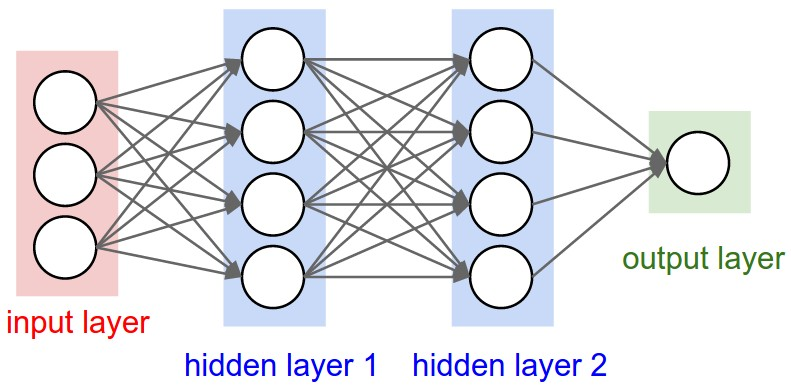
\includegraphics[width=3in]{photo/neural-network}\\
  \caption{A 3-layer neural network with three inputs, two hidden layers of 4 neurons each and one output layer. Notice that in both cases there are connections (synapses) between neurons across layers, but not within a layer.}
  \label{fig:neural-network}
  \end{center}
\end{figure}
%========================================================================
 can solve different types of tasks. Today we had not just the standard neural networks as in the early beginning of there first implementation. Instead, we have more advanced and complicated models. Most of them are designed to solve a specific task, and they are not able to adapt to another category of tasks. For example, Convolution Neuronal networks which are introduced in the \hyperref[subsec:cnn]{Convolutional Neural Network Section} are widespread in the are of image classification. Recurrent neuronal networks are used for text and voice recognition. So, it would not lead in better results if we use and recurrent neural networks which perform very good at text recognition for an image classification task, even then when we had just a convolutional neuronal network that performs not so well.
\subsection{Convolutional Neural Networks}
\label{subsec:cnn}
\noindent To solve the image classification task, we are using a convolutional neuronal network (CNN). Convolutional Neural Networks are a particular case of feed-forward neural networks \cite{Goodfellow-et-al-2016}. . The function of a feed-forward neural network can simply be described as \(y = f(x, \o )\) . CNN's and feed-forward neural networks are estimating parameter values. So for \(y = f(x, \o )\) we estimate the parameter \(\o \) \cite{Goodfellow-et-al-2016}. Through those estimated parameter values we are receiving a function back with the smallest possible difference between the predicted output values and the defined output values. A function that measures the difference between the expected - and the defined output is a so-called loss function \cite{Goodfellow-et-al-2016}. To compare our model accuracy with other model, we are using the following evaluation criteria:
\begin{equation}
Acc(f,D) = \frac{1}{m}\sum_{m}^{i=1} \mathbb{I} \left [ y^{(i)} =f(x^{()i)})\right ]
\label{acc}
\end{equation}
CNN's and classical feed-forward neuronal networks differ in their basis of calculation. Feed-forward neural networks are using matrix multiplication, whereas CNN's are using convolutions. Convolutional layers, pooling layers, and fully-connected layers are specific layers for a CNN \cite{LeCun1998}. \\
\subsubsection{Model Architecture}
\label{subsec:ModelArchitecture}
For our model, we choose pretty much the underlying implementation of the official  website. It is an implementation of an architecture which is introduced by a group of researches which working for Nvidia. Their study showed that it is possible to train a model which can be used for autonomous driving. Especially the researchers showed that Donkeycar is using a small amount of labelled data — more precisely,  only a few pictures from a short time of driving, where the images are marked with the direction in which the vehicle should drive\cite{LearningForSelf-DrivingCars}. As in our \hyperref[sec:LiteratureSurvey]{Literature Survey} mentioned Christian Friedrich Coors implemented the model before.  As he said, the model has 266.628 parameters which can be trained \cite{Coors}. The architecture you can see in Figure \ref{fig:Archi}.
%========================================================================
\begin{figure}
  \begin{center}
  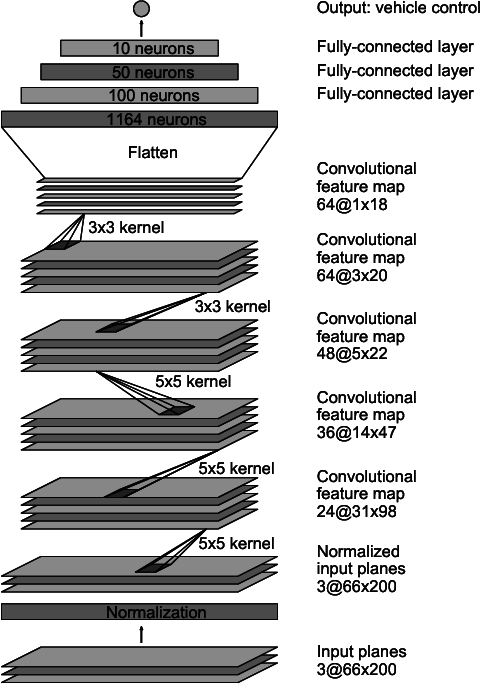
\includegraphics[width=3in]{photo/CNNArchitecture.png}\\
  \caption{Model Architecure from the Nvidia Research Team \cite{LearningForSelf-DrivingCars}}
  \label{fig:Archi}
  \end{center}
\end{figure}
%========================================================================
The Team around Nvidia concluded in their paper that there is more work to do for getting the driving process more stable \cite{LearningForSelf-DrivingCars}. Jelena Kocić and their team focused on this task and got a better result. They reached their goal by using other building blocks like a pooling layer. They mentioned that the training process and the driving process is more computational intense. Because of the few hardware resources of the raspberry pie, we decided to use the first model. \cite{AutomotivePlatformsAutonomousDriving}
\subsubsection{Convolutional Layers}
\noindent The convolutional Layer performs the extracting of features from the input matrix into a feature map. For this procedure, we use matrix multiplication in the form of the dot product and a filter (feature detector, kernel) \cite{Goodfellow-et-al-2016}. 
%========================================================================
\begin{figure}
  \begin{center}
  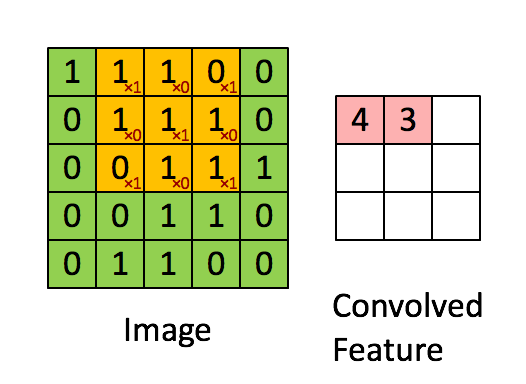
\includegraphics[width=3in]{photo/cnn.png}\\
  \caption{Feature Map derived from http://deeplearning.stanford.edu}
  \label{fig:cnn}
  \end{center}
\end{figure}
%========================================================================
In picture \ref{fig:cnn} can be seen a calculation example of how convolution is applied to a matrix. We are iterating with the filter over the matrix, calculating the scalar product and writing the result into a feature map. An activation function like the rectified linear unit (ReLU) normalizes the feature map after we performed the convolution. Normalization guarantees a feature map which is not a linear transformation of its input value. If this is the case, we only have a linear problem which can be easily solved, but with a wrong results. In other words, the input values get just multiplied by coefficients. Note that there are plenty of reasons for activation functions in a neuronal network. We are giving a closer look at this topic at our section \hyperref[sec:activationFunctions]{"Activation Functions"}. In Figure \ref{featuremap1} you can see how our pictures would change after applying the first convolutional layer. \\
%========================================================================
\begin{figure}
  \begin{center}
  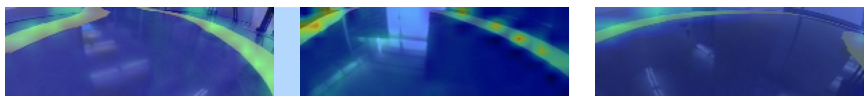
\includegraphics[width=3in]{photo/frist-cl}\\
  \caption{Feature Map from CNN Layer 1}\label{featuremap1}
  \end{center}
\end{figure}
%========================================================================
\begin{figure}
  \begin{center}
  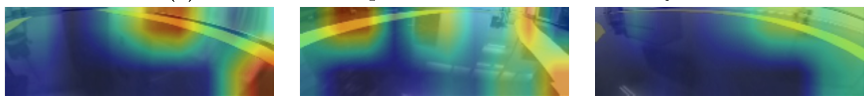
\includegraphics[width=3in]{photo/layer2}\\
  \caption{Feature Map from the last CNN Layer}\label{featuremap2}
  \end{center}
\end{figure}
%========================================================================
This represents the 64 first feature maps of a random picture from the dataset. We can observe that the filters already focus on certain points at the rooms environment. We further used this feature map as input for the second CNN layer. The output of the last feature map u could see in(figure \ref{featuremap2}.\\
\subsubsection{Pooling Layers}
\noindent It is common to add a pooling layer in-between the convolutional layers periodically. The function exists to avoid overfitting and step by step reduce the size of the input image by reducing the number of parameters and computations of the network \cite{RN2}. Anyways as mentioned earlier we decided against pooling layers as discussed in our \hyperref[subsec:ModelArchitecture]{Model Architecture} Section.\\
\subsubsection{Fully-Connected Layers}
\noindent The Dense layer is the last layer of our model. It is also called the \textit{fully connected layer}.  A Dense layer can be seen as a linear operation in which every input is connected to every output by weight. So, there are n inputs multiplied by n outputs weights - which can be a lot — generally followed by a non-linear activation function. This activation functions will then be computed by a matrix multiplication which is followed by a bias offset. 
We are using four of those Dense Layers in our model. The first two Dense Layers are used for Kernel Regularization; the others are used to get the two outputs. We will talk more about the output of our model in the \hyperref[sec:AutonomouslyDriving]{Autonomously Driving} Section. \\
\subsubsection{Kernel Regularization}
\noindent There are many different regularizations to prevent the neural network from overfitting. Next we are going to introduce the two most essential Kernel Regularizations. It can be integrated by penalizing the squared magnitude of all parameters directly in the objective. So, for every weight \textit{w} in the network, the term \(\frac{1}{2} \lambda w^2\) gets added to the objective, where \(\lambda \) is the regularization strength. It's usual to see \(\frac{1}{2}\) in the front, because the gradient of this term with respect to \textit{w} is simply \(\lambda w\) instead of \(2 \lambda w\). The L2 penalizes the peaky weight vectors and prefers the diffuse weight vectors \cite{RN4}. During the gradient descent weight update, the L2 regularization has the meaning, that every weight is decayed linearly (\textit{w += -lambda * w}) towards zero. The Idea of the Drop-Out Kernel Regularisation is to drop out neurons frequently and randomly. That means we are losing Information, but our model is more adaptive to unseen data. The increase in the ability comes from the fact that the weights in dropped out neurons are temporally not updated \cite{Dropout}. In small experiments, the research found out that the younger dropout approach is less computing-intensive and more robust than l2 \cite{dropoutVsL2}. So, we decided - as with the missing pooling layers before - that we are using drop out for Kernel Regularisation to prevent our model for overfitting. \\
\subsubsection{Batch Normalization}
\noindent A technique developed by Ioffe and Szegedy \cite{RN4} is called Batch Normalization properly initializes neural networks by explicitly forcing the activations throughout a network to take on a unit gaussian distribution at the beginning of the training. Normalization is a simple differentiable operation. 
It allows to use higher learning rates at the beginning and is less vulnerable to a bad initialization. In other words, neural networks that implement batch normalization layers are significantly more robust. Additionally, batch normalization can be interpreted as a preprocessing step on every layer of the network. Batch normalization yields in general, a substantial improvement in the training process. \\
\subsubsection{Activation Functions}
\label{sec:activationFunctions}
\noindent There a couple of widely used activation functions like tanh, sigmoid function, ReLU or the ELU. For our model we decided to use the \textit{ReLU} activation function. The Rectified Linear Unit (ReLU) has become very popular in the last few years. It computes the function \(f(x)=max(0,x)\). In other words, the activation is simply thresholded at zero. There are plenty of pro's and con's for the ReLU:
\begin{itemize}
\item (+) Compared to tanh/sigmoid neurons that need to compute expensive operations  like the exponentials, the ReLU can be implemented by directly thresholding a matrix of activations at zero.
\item (+) It was found to notably accelerate the convergence of stochastic gradient descent (SGD) compared to the tanh/sigmoid functions. That is, because of its linear, non-saturating form.
\item (-) Sadly, ReLU units can be weak during training and possibly “die”. For example, a large gradient streaming through a ReLU neuron could cause the weights to update in a dead end, so that it will never activate again. If this happens, then the gradient streaming through the unit will forever be zero. The ReLU units can irreversibly die during training since they can get eliminated off the data manifold. With a good scheduling setting of the learning rate this is less likely to happen. \\
\end{itemize}
\subsubsection{Loss function}
\noindent Our compiled Keras model uses the \textit{cross-entropy-loss} \cite{RN3}. 
\begin{equation}
L_{i} = f_{y_{i}} + log \sum_{j} e^{f_{j}}
\end{equation}
where we are using the notation \(f_{j}\) to mean the \textit{j-th} element of the vector of class scores \textit{f}. The full loss for the dataset is the mean of \(f_{i}\) over all training examples together with a regularization term \textit{R(W)}.
The cross-entropy loss, or also called log loss, measures the performance of our classification model with the output as probability values between zero and one. The cross-entropy loss increases as the predicted probability diverges from real value labels.
\subsubsection{Optimizer}
\noindent There are many possible optimizer suitable for our task. The common ones are the RMSprob, Adam or the stochastic gradient descent (SGD) \cite{RN1}. As before at our Section about kernal regularization we are going to introduce the two most essential Ways to Optimize our Model. While doing an Image classification with 10 Classes as in cifar10, we could decide to use the SGD to minimize the loss by computing the gradient with respect to a randomly selected batch from the training set. This method is more efficient than computing the gradient with respect to the whole training set before each update is performed. 
\begin{equation}
\frac{\partial p_i}{\partial a_j}=\left\{\begin{matrix} p_i(1-p_i) & if & i=j\\ -p_j p_i & if & i\neq j \end{matrix}\right.
\end{equation} \\
\begin{equation}
\frac{\partial L}{\partial o_i}=p_i-y\_oh_i
\end{equation} 
For the derivation of the cross entropy loss, \textit{y\_oh} is the one-hot encoded representation of the class labels. But in our case we decied to use the Adam optimizer. An even more efficient optimizer. Research found out that it is compared to other opimizer a better perfomer in every aspect \cite{AutomotivePlatformsAutonomousDriving} \cite{Adam}
\subsubsection{Softmax}
\noindent The softmax normalizes the class probabilities to one and it has a probabilistic interpretation. 
\begin{equation}
f_{j}(z) = \frac{e^{z_{i}}}{\sum_{k} e^{z_{k}}}
\end{equation}
The exponential values can very quickly explode to an infinite large number, for example \(e_{1000}\). To fix this issue, it takes a one-dimensional vector of arbitrary length (in \textit{z}) and puts it into a vector of values between zero and one that sum together to one. The cross-entropy loss that includes the softmax function, hence to minimize the cross-entropy-loss between the estimated class probabilites. \\
\subsubsection{Flatten}
In between the convolutional layer (CNN) and the fully connected layer (Dense), there is a \textit{Flatten layer}. The Flattening layer transforms a two-dimensional matrix of features into a one-dimensional vector that can be respectively streamed into the fully connected neural network classifier, which are our ten fully connected animal neurons. \\


\section{Autonomously Driving}
\label{sec:AutonomouslyDriving}

At this point our car is equipped with a fully trained model and is ready to drive. Since our neuronal network is build with Keras, the Raspberry Pi uses the KerasPilot-Part to load the trained model and evaluate the captured pictures with that respectively. The pictures captured by the PiCamera are 160x120 pixels with 3 color channels (red, green, blue). The CNN layers which the image need to pass through are shown in figure \ref{cnn_table}.

\begin{figure}
  \begin{center}
  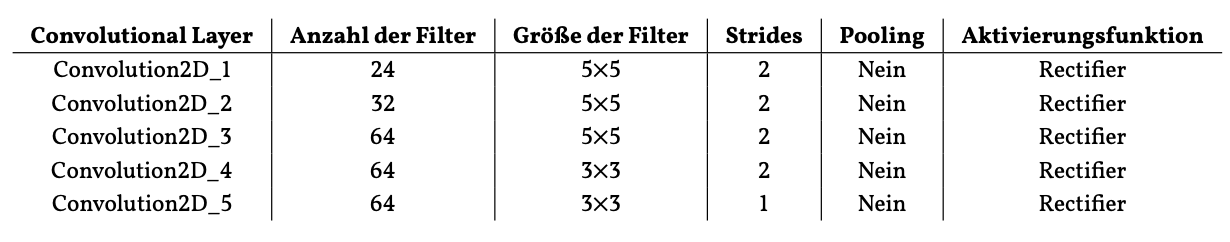
\includegraphics[width=3.5in]{photo/cnn_table.png}\\
  \caption{CNN Table}\label{cnn_table}
  \end{center}
\end{figure}

The network produces two different outputs:

\begin{itemize}
\item angle\_out: as PWM signal
\item throttle\_out: for the car speed
\end{itemize}

The car speed can be set manually to a constant value. This is especially useful when we let the car drive indoors, because it cannot speed up so much as outdoors. So for our case we only depend on the angle\_out output. The High-Level-Bibliography is Keras, which is accordingly based on Tensorflow. For our project we use Tensorflow 1.0, not the latest release 2.0. \\

\begin{figure}
  \begin{center}
  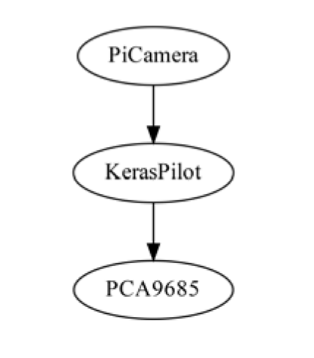
\includegraphics[width=1.3in]{photo/autonom.png}\\
  \caption{Graph of Dataflow}\label{autonom}
  \end{center}
\end{figure}

As already mentioned in \hyperref[cameramodule]{section PiCamera}, we use 20 FPS, so we receive 20 angle\_out outputs per second. This calculations are processed on the Raspberry Pi and the values are directly transmitted to the PCA9685 servodriver and then to the servomotor of the car. This is why the car shakes often while driving, because it receives so many new values where it needs to steer its angle.


\section{Evaluation}

Even though CNN perform a really good result in the computer vision field, it is still quite hard to decompse the decisions and the filters to understand the blackbox behind. Especially in the image recognition the filter decide randomly on which shapes and particles it is going to focus. By adding more and more layers to the neural network we make it harder and harder to interpret the parameters. In the case of a fail it is going to be very hard to evaluate the misstakes e.g. overfitting, underfitting, too much noise in the data or the task might even be too complex for the neural network. We are able to visualize the filter after for example the first filter of the convolutional neural network shown in figure \ref{filter}. It is useful to illustrate this filter, because the visualized noise could make a overfitting visible in the image. \\

\subsubsection{Occlusion Maps}
\begin{figure}
  \begin{center}
  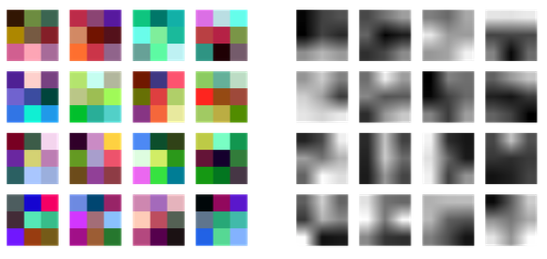
\includegraphics[width=3.5in]{photo/filter.png}\\
  \caption{Color not interpolated filter and grayscale filter with bilinear interpolation \cite{master}}\label{filter}
  \end{center}
\end{figure}

To evaluate the convolutional neural network with occlusion maps, we set the criterion function based on if the car drives within the lanes. Since we do not use a middle-lane, but only two lanes for the border, the autonomous car should identify correctly the two border-lines. The criterion function looks like the following:

\[
    O_{i,j}= 
\begin{cases}
    0,& \text{if } abs(\hat{y}_{i,j} - y) > \epsilon\\
    1              & \text{otherwise}
\end{cases}
\]

Where y is the angle predicted from the neural network without any occlusion and \^{y} is the regressed angle when the center of the occluding rectanle is placed at location (i, j) of the input image \cite{master}. We do not need any deeper knowledge of the neural networks architecture to understand this straight-forward process, because we only use the networks output. One of the disadvanteges of this technique is that we need to evaluate a lot of different picture to detect the important features of the image.

\subsubsection{Visualizing Activations}

Another easy way to evaluate our model is to show each layer's activation after every convolution. We can compute with by multiplying the the trained filters with the input data and apply the activation function onto it, for example ReLU. We get a more and more decreased set of features after each layer of the neural network. We are able to extract those activations and display them (figure \ref{activations}) as picture with the python package \textit{matplotlib}. 

\subsubsection{Occlusion Maps}
\begin{figure}
  \begin{center}
  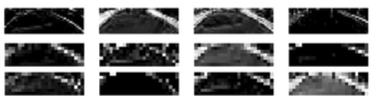
\includegraphics[width=3.5in]{photo/activations.png}\\
  \caption{Activation features after each Layer of the NN  \cite{master} }\label{activations}
  \end{center}
\end{figure}

\section{Conclusion}
As we finished the last challenge of this hard project, a feeling of relief overcame every member. It was intellectually - and all of us agree on this - one of the most difficult tasks we encountered as students. We had to face more difficulties than we expected. In the end we were very happy of the successful outcome though.
<<<<<<< HEAD
Obviously the group spirit dependent whether the daily objectives we set were successfully reached or not. Especially in the beginning, when we did not really no how to tackle the faced problems, we were constantly nervous and in  bad mood. The closer we came to something we call a success the better was our mood. The first time we saw the car driving on its own around the corner, we were happy for days.
We also grew together as a team. The delegation of the tasked happened according to our strengths and weaknesses. Before the project we knew each other, but we can say that after the project we know each other way better than before.
The timespan given to us from the university of two semester was sufficient for accomplishing the main objective. The so called supervised learning on our neuronal networks was successful. For the other way to train the network, the so called reinforcement learning, the given time and/or experience we had with this technology, was not enough. Therefore we conducted a “literature survey” where we evaluated other projects which used reinforcement learning technology and analysed whether the given technology could be implemented in our project or not. 
=======
We grew together as a team. The delegation of the tasked happened according to our strengths and weaknesses. Before the project we knew each other, but we can say that after the project we know each other way better than before.
The timespan given to us from the university of two semester was sufficient for accomplishing the main objective. The supervised learning on our neuronal networks was successfully tested. Originally we planned to experiment regarding unsupervised learning (Reinforcement Learning), but the given timespan was not sufficient enough for this extended project and the complexity was higher than expected. Therefore we conducted a “literature survey” where we evaluated other projects which used reinforcement learning technology and analysed whether the given technology could be implemented in our project or not. 
>>>>>>> 51a751091ea4275a0407352401eaf8d9d9b0d98e
We learned the sophisticated interaction between different hardware components and the different software which run on them. Furthermore we got an good overview of the state of the art technology of machine learning software in general.
Two of three members will definitely try to get a job in this area. They applied for jobs or already have a job where they have to analyse or manipulate big amounts of data.

\section*{Acknowledgment}
\noindent The authors would like to thank Prof Dr. Florian Gallwitz from the University of Applied Science - Georg Simon OHM in Nuremberg for a really good supervising of our group. 



% if have a single appendix:
%\appendix[Proof of the Zonklar Equations]
% or
%\appendix  % for no appendix heading
% do not use \section anymore after \appendix, only \section*
% is possibly needed

% use appendices with more than one appendix
% then use \section to start each appendix
% you must declare a \section before using any
% \subsection or using \label (\appendices by itself
% starts a section numbered zero.)
%

% ============================================
%\appendices
%\section{Proof of the First Zonklar Equation}
%Appendix one text goes here %\cite{Roberg2010}.

% you can choose not to have a title for an appendix
% if you want by leaving the argument blank
%\section{}
%Appendix two text goes here.


% use section* for acknowledgement
%\section*{Acknowledgment}


%The authors would like to thank D. Root for the loan of the SWAP. The SWAP that can ONLY be usefull in Boulder...


% Can use something like this to put references on a page
% by themselves when using endfloat and the captionsoff option.
\ifCLASSOPTIONcaptionsoff
  \newpage
\fi



% trigger a \newpage just before the given reference
% number - used to balance the columns on the last page
% adjust value as needed - may need to be readjusted if
% the document is modified later
%\IEEEtriggeratref{8}
% The "triggered" command can be changed if desired:
%\IEEEtriggercmd{\enlargethispage{-5in}}

% ====== REFERENCE SECTION

%\begin{thebibliography}{1}

% IEEEabrv,

\bibliographystyle{IEEEtran}
\bibliography{Bibliography}
%\end{thebibliography}
% biography section
% 
% If you have an EPS/PDF photo (graphicx package needed) extra braces are
% needed around the contents of the optional argument to biography to prevent
% the LaTeX parser from getting confused when it sees the complicated
% \includegraphics command within an optional argument. (You could create
% your own custom macro containing the \includegraphics command to make things
% simpler here.)
%\begin{biography}[{\includegraphics[width=1in,height=1.25in,clip,keepaspectratio]{mshell}}]{Michael Shell}
% or if you just want to reserve a space for a photo:

% ==== SWITCH OFF the BIO for submission
% ==== SWITCH OFF the BIO for submission


%% if you will not have a photo at all:
%\begin{IEEEbiographynophoto}{Ignacio Ramos}
%(S'12) received the B.S. degree in electrical engineering from the University of Illinois at Chicago in 2009, and is currently working toward the Ph.D. degree at the University of Colorado at Boulder. From 2009 to 2011, he was with the Power and Electronic Systems Department at Raytheon IDS, Sudbury, MA. His research interests include high-efficiency microwave power amplifiers, microwave DC/DC converters, radar systems, and wireless power transmission.
%\end{IEEEbiographynophoto}

%% insert where needed to balance the two columns on the last page with
%% biographies
%%\newpage

%\begin{IEEEbiographynophoto}{Jane Doe}
%Biography text here.
%\end{IEEEbiographynophoto}
% ==== SWITCH OFF the BIO for submission
% ==== SWITCH OFF the BIO for submission



% You can push biographies down or up by placing
% a \vfill before or after them. The appropriate
% use of \vfill depends on what kind of text is
% on the last page and whether or not the columns
% are being equalized.

\vfill

% Can be used to pull up biographies so that the bottom of the last one
% is flush with the other column.
%\enlargethispage{-5in}



% that's all folks
\end{document}
